\author{Florian Müller}
\section {Finding Checkboxes}

\texttt{answer, image = find\_checkboxes(picture, roi, task:Task, correcting:bool)}

The main function from the checkboxchecker package is \texttt{find\_checkboxes()}.
This function will receive four arguments and output a list of checked boxes and a colored image of the roi.

In the begining of the function the line thickness and fontsize will be calculated for the size of the picture.
Also the colors which are used are defined.

Then the roi will be cut from the original picture.

\begin{figure}[H]
    \centering
    \begin{minipage}[b]{.4\linewidth}
        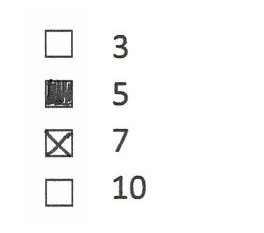
\includegraphics[width=\linewidth]{src/chapters/developer/media/cbc_live/cbc_roim.png}
        \caption{Region of interesst}
    \end{minipage}
\end{figure}

Convert the roi to grayscale.

\begin{figure}[H]
    \centering
    \subfloat[][]{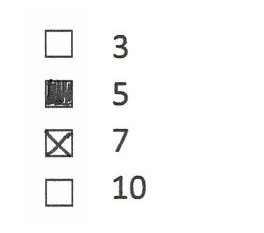
\includegraphics[width=0.4\linewidth]{src/chapters/developer/media/cbc_live/cbc_roim.png}}
    \qquad
    \subfloat[][]{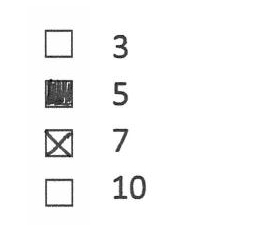
\includegraphics[width=0.4\linewidth]{src/chapters/developer/media/cbc_live/cbc_grey.png}}
    \caption{From original(a) to grayscale(b)}
\end{figure}

Blur the image to get rid of possible little holes in it.

\begin{figure}[H]
    \centering
    \subfloat[][]{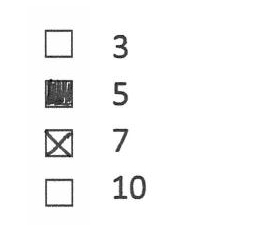
\includegraphics[width=0.4\linewidth]{src/chapters/developer/media/cbc_live/cbc_grey.png}}
    \qquad
    \subfloat[][]{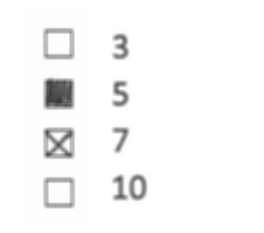
\includegraphics[width=0.4\linewidth]{src/chapters/developer/media/cbc_live/cbc_blurgrey.png}}
    \caption{From grayscale(a) to blured(b)}
\end{figure}

Threshold the image.

\begin{figure}[H]
    \centering
    \subfloat[][]{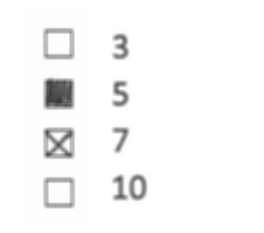
\includegraphics[width=0.4\linewidth]{src/chapters/developer/media/cbc_live/cbc_blurgrey.png}}
    \qquad
    \subfloat[][]{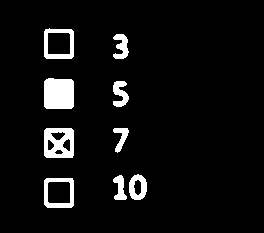
\includegraphics[width=0.4\linewidth]{src/chapters/developer/media/cbc_live/cbc_thresh.png}}
    \caption{From blured(a) to threshed(b)}
\end{figure}

Find the contours and iterate of each contour to determine if it is a checkbox.
Each checkbox which is found will be added to the checkbox list.

If it is in the correcting mode the actual answers will be read out of the task.
Again an iteration over every checkbox and a check with \texttt{\_countCheckboxPixels()} if the box is checked, empty or filled.

After that all boxes will be colored and the found filling is written to the boxes.

\begin{figure}[H]
    \centering
    \subfloat[][]{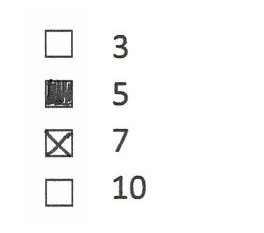
\includegraphics[width=0.4\linewidth]{src/chapters/developer/media/cbc_live/cbc_roim.png}}
    \qquad
    \subfloat[][]{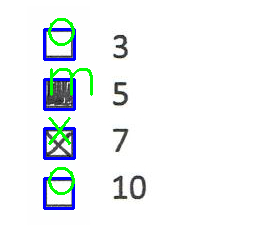
\includegraphics[width=0.4\linewidth]{src/chapters/developer/media/cbc_live/cbc_drawing.png}}
    \caption{From original(a) to coloerd(b)}
\end{figure}

In the end the list with the answers and the drawing will be returned.

